\chapter{Referencial Teórico}
\label{cap-referencial}

\section{Implantação de Software}

Software só oferece valor para os clientes quando eles estão implantados em produção
e assim possam proporcionar as funcionalidades necessárias ao usuário final,
por isso a importância da fase de implantação de software, pois é nela em que a equipe
de desenvolvimento disponibilizará o software ou uma atualização com novas funcionalidades
ao usuário. Sendo assim, a Implantação de software é um conjunto de atividade cruciais
para todos os fornecedores de software, isto começa desde um pedido de um novo requisito
de software até todas as medidas necessárias para essa nova versão está disponível
para o cliente \cite{5741269}. A implantação de software é composta com várias
atividades que são essenciais para disponibilizar um produto a alguém, como por exemplo:
instalação de dependências, arquivos de configuração e instalação da própria aplicação.

De acordo com \cite{deployment1998} as aplicações de software não são mais
sistemas autônomos, são cada vez mais o resultado da integração de coleções de
componentes, o que pode tornar a implantação de software um processo complicado, e
nem sempre existir a garantia de que cada componente será implantado corretamente.
Portanto, a equipe de desenvolvimento deve encontrar uma maneira de lidar
com uma maior incerteza no ambiente nos quais seus sistemas vão operar, garantindo
que a implantação do software seja feita da forma correta, evitando quaisquer acontecimentos
de erros e imprevistos.

Uma grande aliada das equipes de desenvolvimento é a implantação automatizada de
software, que se refere à prática de implantar o software para os usuários finais
automaticamente, evitando qualquer tipo de execução de esforço manual, por isso
a prática de implantação automatizada facilita na rápida entrega de software, tanto
para implantações de aplicações em servidores na nuvem, como implantação de software
para usuários em seus computadores.\cite{7284592}.

Todas essas questões devem ser levadas em consideração e a atividade de implantação de
software deve receber uma atenção especial, visto que os softwares estão ficando
cada vez mais complexos, podendo ter várias ferramentas integradas em diferentes
linguagens de programação e diferentes configurações, com todas essas variáveis compondo
uma implantação automatizada de software. Este capítulo possui uma subseção sobre
processo de Implantação de Software, para entender melhor como funciona o processo de implantação
de software, depois uma subseção sobre DevOps, que busca trazer um conceito de implantação
automatizada de software junto aos métodos ágeis, e por fim, uma subseção sobre
ferramentas e técnicas que buscam facilitar e resolver os problemas da
implantação automatizada de software, com as características típicas que essas
ferramentas trazem para tornar a implantação mais rápida e com qualidade.

\subsection{Processo de Implantação de Software}

A implantação de um software é o processo que vai desde a aquisição desse software
até a sua execução \cite{leo2014}. O processo implantação consiste em diversas
atividades que devem ser executadas desde o planejamento da implantação até a
disponibilidade para uso.

A OMG (Object Management Group) é uma organização internacional sem fins lucrativos
que aprova padrões abertos para tecnologias e eles definem uma especificação de
implantação e configuração de aplicações distribuídas baseadas em componentes \cite{omg2006},
a OMG também diz que o processo de implantação é um processo que se inicia desde
a aquisição de um componente até o momento em que esse componente está em plena
execução, pronto pra uso.

Segundo \cite{omg2006} os principais termos definidos dentro de uma implantação
de software são:

\begin{itemize}
  \item  \textbf{Implantador:} Pessoa ou equipe responsável pelo processo de
  implantação  de um sistema.
  \item  \textbf{Ambiente alvo:} São o servidor ou conjunto de servidores em
  que os componentes são implantados.
  \item  \textbf{Nó:} É um recurso computacional onde se implanta um componente,
  por exemplo uma máquina virtual dentro do servidor que vai hospedar um serviço
  de banco de dados. Os nós fazem parte do ambiente alvo.
  \item  \textbf{Pacote:} Artefato executável que contém o código binário do componente
  . É por meio de um pacote que um serviço pode ser instalado e executado dentro
  de um sistema operacional, e que são característicos dependendo da distribuição
  do sistema operacional, por exemplo: .deb para debian e .rpm para redhat, ou
  pacotes independentes de sistema operacional como: jar.
\end{itemize}

Além disso, é definido as fases que compõem o processo de implantação e de acordo
com \cite{omg2006} as fases são:

\begin{itemize}
  \item  \textbf{Planejamento:} O planejamento da implantação é uma fase
  para identificar os componentes necessários na implantação e como cada um será
  distribuído entre os nós do ambiente alvo.
  \item  \textbf{Preparação:} São os procedimentos necessários para preparar o
  ambiente alvo para que um determinado componente possa ser executado, isso envolve
  configuração do sistema operacional, instalação e configuração de dependências
  necessárias (por exemplo um servidor web como apache ou nginx) e a transferência
  do componente para o servidor onde ele será executado.
  \item  \textbf{Instalação:} O implantador transfere o componente para a infraestrutura
  alvo, é quando instalamos um dado componente em um servidor, um exemplo disso
  é a instalação de uma aplicação via pacotes (.deb ou .rmp).
  \item  \textbf{Configuração:} Edição de arquivos de configuração para alterar
  determinado comportamento de uma aplicação, o implantador aplica configurações
  específicas a aplicação a partir de arquivos de configuração.
  \item  \textbf{Inicialização:} É quando a aplicação é iniciada e entra em execução,
  pronto para receber chamadas de seus clientes.
\end{itemize}

Os termos e fases formam uma estrutura básica que um processo de implantação de software
deve conter, podendo haver modificações de acordo com a necessidade do implantador,
cada fase é necessária para que possa ter uma implantação consistente, ou seja, as
atividades dentro de uma implantação de software estarão organizadas, evitando assim
possíveis erros durante a implantação, essa organização também podendo ajudar o
time de implantação a encontrar os problemas ocorridos dentro de uma implantação
de software, caso ocorram.

Dependendo do tamanho da aplicação essas fases podem se tornar tarefas complicadas,
com isso existe a necessidade de automatizar o processo de implantação, assim
diminuindo a possibilidade de erros comparado a uma tarefa manual e consequentemente
tornando o trabalho mais ágil, dando adeus aos longos manuais de instalação.
\cite{humble2010} diz que o objetivo de um processo de implantação automatizado é
proporcionar um processo de implantação reprodutível, confiável e fácil de ser
executado.

Para que a implantação automatizada de software seja possível, é necessário o uso
de ferramentas para poder automatizar todo o processo de implantação,
mas é necessário que o implantador compreenda cada fase do processo para que possa ser
feito um bom planejamento e execução da implantação.

\subsection{Introdução ao DevOps}
\label{subsec:DevOps}
Como resultado ao longo dos anos, o que aconteceu é que as equipes de desenvolvimento de software
são capazes de entregar a um ritmo muito mais rápido, principalmente a adoção
de métodos ágeis de desenvolvimento de software \cite{7173368}, como podemos
ver na figura \ref{fig:DevOps}, as equipes desenvolvem de forma acelerada, enquanto
a equipe de operações consegue implantar de forma sequencial. Sendo assim DevOps
nasceu a partir dessa necessidade de implantar software no mesmo ritmo em que
as equipes são capazes de entregar novas funcionalidades.

\begin{figure}[h]
  \centering
  \caption{Fluxo de desenvolvimento de software em relação a implantação}
  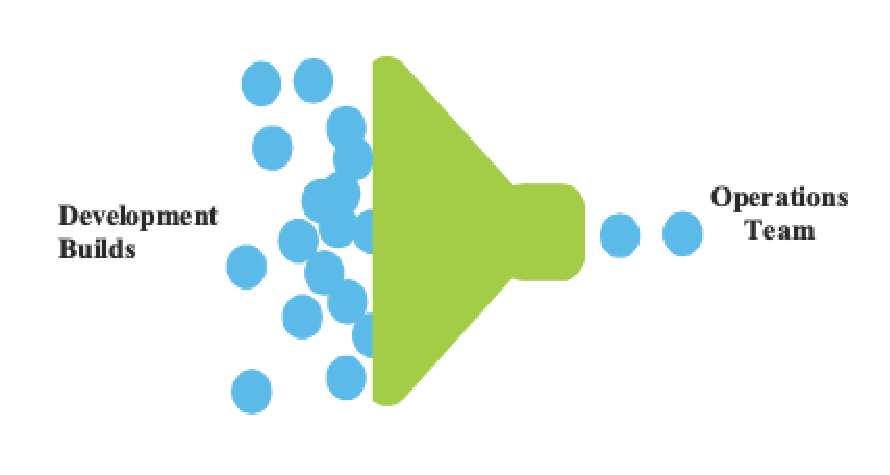
\includegraphics[width=1.0\textwidth]
      {figuras/devops.eps}
    Fonte: \cite{7173368}
\label{fig:DevOps}
\end{figure}

DevOps pode ser visto como um conjunto de práticas e princípios para a entrega de software, onde a
chave é o foco e a velocidade de entrega e automação, para pode auxiliar na capacidade
de reagir a mudanças \cite{7173368}. A automação da implantação de software vem
principalmente pela necessidade do alinhamento entre o time de desenvolvimento
com o time de operações. Essa necessidade vem em relação a ligação entre as duas
equipes em relação ao processo de implantação de software, ferramentas para
automatizar implantações de software, as atividades de implantação e responsabilidades
dentro do ciclo de desenvolvimento, o que antes não era visto, o que acontecia é
que o time de desenvolvimento terminavam suas funcionalidades e seus testes e
entregavam a uma equipe de implantação. DevOps tenta unir esses dois mundos,
fazendo com que as duas equipes compartilhem atividades e responsabilidades \cite{6265084}.

De acordo com \cite{httermann2012DevOps} a comunidade DevOps defende a comunicação
entre a equipe de operações e a equipe de desenvolvimento como um meio de assegurar
que o os desenvolvedores entendam os problemas associados com as operações. Um dos
principais benefícios disso é a capacidade de quantificar aspectos do desenvolvimento,
isto é, levar a melhoria do desenvolvimento do produto, devido a um foco mais nítido
em agilidade das entregas.

Em \cite{7173368} é abordado as práticas DevOps, que podem ser aplicadas diversas
 vezes dentro de um ciclo de desenvolvimento de software, as praticas DevOps podem ser resumidas em:

 \begin{itemize}
   \item \textbf{Planejamento Contínuo:} O planejamento deve ser sempre contínuo
   e evoluindo junto ao planejamento da equipe de desenvolvimento, com tarefas
   sendo priorizadas o tempo todo e sempre alinhadas de acordo com as decisões tomadas
   em conjunto com a equipe de desenvolvimento.
   \item \textbf{Integração Contínua:} Compartilhar as alterações feitas com toda equipe
   evitando que as novas modificações fiquem apenas nas mãos do time de desenvolvimento.
   \item \textbf{Implantação Contínua:} O coração do DevOps, recomenda-se automatizar
   todo o processo de implantação, removendo quaisquer tipo de etapas manuais com auxílio
   de uma ferramenta que possa automatizar a instalação, sendo assim a implantação
   de cada nova versão de software passa a ser de forma mais rápida e eficiente.
   \item \textbf{Testes Contínuos:} Automatiza também os testes da sua aplicação.
   \item \textbf{Monitoração Contínua:} Monitorar as novas alterações
   que foram implantadas a fim de aumentar a capacidade de reagir a quaisquer surpresas
   em tempo hábil.
 \end{itemize}

 Os benefícios do uso do DevOps são vários, como por exemplo: economia de tempo,
 já que implantação de software passa a ser um processo natural, economia de custos, aumentar
 a organização e eficiência do desenvolvimento de software como um todo \cite{7173368}.

Para a entender melhor a prática de implantação automatizada, que é o coração
do DevOps, é necessário possuir um conhecimento prévio sobre ferramentas para
automatizar a implantação de software, conhecendo algumas ferramentas utilizadas
no mercado para automatizar implantação e suas maneiras de atuação, além das técnicas
de implantações utilizadas, como por exemplo o empacotamento de software.

\subsection{Métodos e ferramentas para implantação automatizada de software}
\label{subsec:metodoseferramentas}

%empacotamento, instalação via script, tar.gz, exe, jar, etc.

Existem várias maneiras de se automatizar um processo de implantação software,
de acordo com \cite{leo2014}, podem-se utilizar linguagens de script de propósito
geral como (Python, shell script), ferramentas gerais voltados para o processo
de implantação ou sistemas de middleware especializados em determinados tipos de artefatos implantáveis.
Um processo de implantação automatizado depende bastante da integração de diferentes papéis
em uma organização, foi dito também na seção \ref{subsec:DevOps} que é importante a
integração entre desenvolvedores e operadores, uma vez que o desenvolvimento desses
scripts ou utilização das ferramentas precisam de participação de ambos os perfis.

Existem várias soluções técnicas  para melhorar a implantação de software \cite{5741269},
no entanto, apesar da sua importância para as empresas de software, as atividades
de implantação de software têm recebido pouca atenção. Em \cite{deployment1998}
é dito que recentemente, um número de novas tecnologias começaram a emergir para
resolver o problema de implantação. As características típicas oferecidas por
estas tecnologias incluem sistemas para automatizar a implantação a partir de
configurações, pacotes, gerenciamento de rede e instalação de recursos, com
propósito de entrega das atualizações de forma automática.

Assim, um grande facilitador da implantação de software são as ferramentas que auxiliam na
automação das atividades de implantação, pois dependendo do software, a implantação
pode se tornar um processo com muitas atividades ou bastante longo, e a automação
vêm para facilitar a implantação, evitando erros de instalações manuais e facilitando a replicação em
vários ambientes diferentes.

De acordo com \cite{6265084} tais ferramentas permitem-nos controlar e automatizar
a configuração de todos os elementos que compõem um sistema, são eles: hosts, software a serem instalados,
usuários do sistema, serviços em execução, arquivos de configuração, tarefas agendadas,
configuração de rede, armazenamento de arquivos, monitoramento e segurança. Existem
ferramentas populares como Puppet e Chef, tendo como sua principal função principal
de automatizar a instalação e configuração de um sistema. Com essas ferramentas é
possível escrever algumas regras que expressam como um software deve ser configurado,
e assim a ferramenta configurarará o sistema conforme as especificações.

Essas ferramentas funcionam de forma declarativa, especificando a instalação de um sistema de
através de regras \cite{6265084}. Por exemplo, é possível especificar regras para a configuração do sistema
a partir de uma infraestrutura básica, no chef essa estrutura é conhecida como livro
de receitas, em puppet essa estrutura é conhecida como manifesto, esses recursos
são basicamente arquivos, no qual o implantador define os passos que serão executados,
cada um podendo executar: um aplicativo, um serviço, papéis de usuários do sistema,
aruivos de configuração e etc.

Cada passo da configuração desejada pode depender de outros passos, ou seja, para
instalar uma aplicação é preciso instalar previamente um compilador ou interpretador da linguagem,
um exemplo é que para rodar uma aplicação web é necessário a instalaçã prévia de
um servidor web. Para lidar com estas dependências essas ferramentas descrevem o estado em que a aplicação
deve estar, ou seja, todos os pacotes, arquivos de configuração diretórios e usuários,
sendo possível definir a dependência entre as tarefas a serem executadas.

Com essas ferramentas a implantação de um software dentro de uma infraestrutura
não precisa ser um esforço manual, com elas podemos automatizar toda a implantação
de um software, desde a preparação do ambiente até a inicialização da aplicação,
sendo assim possível reduzir o tempo gasto na implantação, sem qualquer esforço
adicional, o que integra os conceitos de DevOps com implantação de software automatizada
de software.

Além das ferramentas de automação, é importante também entender o empacotamento de
programas, tanto chef como puppet utilizam a instalação de pacotes como recurso para
poder instalar softwares, ou seja, é possível buscar os softwares desejados a partir
dos pacotes disponíveis em uma distribuição linux. As distribuições linux que
optam por disponibilizar pacotes mantém uma infraestrutura de servidores como fonte
de distribuição de programas \cite{araujo2011apprecommender}, tais servidores são
chamados de repositórios, e esses pacotes são gerenciados com softwares conhecidos
como sistemas gerenciadores de pacotes, que possuem a responsabilidade de buscar
os softwares a serem instalados que estão disponíveis nos respectivos repositórios.

Existem pacotes que dependem do sistema operacional, como por exemplo, pacotes .deb
para a distribuição Debian e pacotes .rpm para a distribuição Fedora, e
pacotes independentes de sistema operacional, como por exemplo, pacotes jar da
linguagem java. Neste trabalho trataremos apenas de pacotes Debian.

\subsubsection{Pacotes Debian}

O formato utilizado pelo Debian GNU/LINUX e seus derivados é o formato de pacotes
binários conhecido como .deb, um pacote .deb é composto de arquivos executáveis,
bibliotecas e documentação associada a um programa ou a um conjunto de programas,
além de todos os dados e procedimentos necessários para instalar, configurar e remover
aplicativos de um sistema \cite{araujo2011apprecommender}. A estrutura dos pacotes
e também os seus requisitos para que sejam distribuídos oficialmente pelo Debian
estão especificados no Manual de Políticas do Debian \cite{debian}.

A estrutura de um pacote debian pode ser observado a partir de qualquer pacote
.deb, onde é possível encontrar três estruturas a seguir:

\begin{itemize}
  \item \textbf{debian-binary:} Este arquivo contém a versão da especificação
  do empacotamento implementado no pacote, em 2015 a versão é a 2.0 nos pacotes.
  \item \textbf{control.tar.gz:} Este arquivamento contém todas as informações
   disponíveis, como o nome e a versão do pacote. Essas informações servem para
   que as ferramentas de gerenciamento de pacotes determinarem se é possível
   instalar e desinstalar o pacote.
   \item \textbf{data.tar.gz:} Este arquivamento contém todos os arquivos para
   serem extraídos do pacote, ou seja, é onde ficam os arquivos executáveis, a documentação,
   os devidos diretórios em que tais arquivos devem ser copiados e etc.
\end{itemize}

Ao instalar um pacote .deb, são feitos todos os procedimentos necessários para a instalação
de uma aplicação, porém, existem ainda casos em que o usuário precise fazer algumas
configurações, um exemplo é quando o usuário precisa configurar um banco de dados
ou fazer uma configuração específica de uma aplicação a partir de arquivos de configuração.
Essas tarefas não são de responsabilidade dos pacotes e sim do usuário que deseja utilizar esse
software, já que o pacote não poderia prever qual é a estrutura e a configuração
que o usuário pretende utilizar, logo a execução desses passos são feitas de
acordo com a preferência do usuário, podendo ser feita manualmente ou a partir
de uma implantação automatizada que utilize alguma ferramenta para isso. Um exemplo
desse tipo de atividade que não é de responsabilidade de um pacote é a configuração
de hospedagem virtual, que será visto na subseção a seguir.

\subsection{Múltiplas Instâncias de Aplicações Web com Hospedagem Virtual}
%falar sobre

Na implantação de software deve-se escolher um ambiente alvo, onde a aplicação
será instalada, esse ambiente deve possuir um nó, que é um recurso computacional
onde se implanta um componente, como por exemplo: uma máquina virtual. Porém pode
existir a necessidade de implantar várias aplicações no mesmo servidor, e no caso
de aplicações web isso pode ser um problema, visto que as aplicações estarão em um
único servidor, assim também em um único IP, que é o número que o servidor recebe
ao se conectar na internet.

Uma forma de solucionar esse problema é o uso de Hospedagem Virtual, de acordo com
\cite{apachevh} hospedagem virtual é um termo que se refere à prática de executar
mais de uma aplicação web em uma única máquina. Com a Hospedagem Virtual é possível
hospedar mais de um nome de domínio no mesmo computador, o que significa que você
tem vários nomes em execução em um único endereço de ip, possibilitando que em um
mesmo servidor você possa ter uma aplicação em www.blog.com e www.nuvem.com. O fato
de que eles estão em execução no mesmo servidor físico não é aparente para o usuário final. Essa
solução é importante para economizar recursos, já que não será necessário possuir
um servidor dedicado apenas a uma aplicação.

Alguns softwares possuem suporte para a implementação de hospedagem virtual, como por
exemplo o Acpahe e o Nginx, o funcionamento de ambos é a partir de arquivos que
especificam a configuração da hospedagem virtual e determina como o servidor
irá responder às várias requisições de domínio. No apache o arquivo padrão de configuração
é chamado 000-default.conf que pode ser utilizado como referência, como por exemplo:

\begin{lstlisting}[language=Xml,label=dice_index,caption={Exemplo de arquivo de configuração de hospedagem virtual no apache}]
  <VirtualHost *:80>
      ServerAdmin webmaster@localhost
      DocumentRoot /var/www/html
      ErrorLog ${APACHE_LOG_DIR}/error.log
      CustomLog ${APACHE_LOG_DIR}/access.log combined
  </VirtualHost>
\end{lstlisting}

Isso quer dizer que as requisições na porta 80 vindas de webmaster@localhost serão
direcioanadas aos arquivos que estão em /var/www/html. Já no Nginx a configuração
de hospedagem virtual também é feita através de arquivos de configuração, o arquivo
padrão no Nginx é chamado de default.conf que também pode ser utilizado como
referência, como por exemplo:

\begin{lstlisting}[language=Ruby,label=dice_index,caption={Exemplo de arquivo de configuração de hospedagem virtual no Nginx}]
  server {
         listen   80; ## listen for ipv4; this line is default and implied
         #listen   [::]:80 default ipv6only=on; ## listen for ipv6

         root /var/www/example.com/public_html;
         index index.html index.htm;

         # Make site accessible from http://localhost/
         server_name example.com;
  }
\end{lstlisting}

Isso quer dizer que as requisições que são ouvidas da porta 80 serão direcionadas
aos arquivos que estão em /var/www/example.com/public\_html, também é indicado o
arquivo index que será o arquivo da página inicial do nome do servidor na porta 80,
além disso é definido example.com para o nome servidor. Além disso existem vários
outros recursos que essas ferramentas possuem, como por exemplo o recurso de proxy,
porém para este trabalho será necessário apenas o uso de hospedagem virtual.

\subsection{Segurança na Implantação de Aplicações Web}
\label{sec:seguranca}

Como vimos, um pacote cumpre bem suas responsabilidades dentro de uma implantação de
software, porém outras atividades também são importantes e que fogem da responsabilidade
de um pacote, outro fator importante é que um pacote também não pode prever é quais são
os procedimentos de segurança que devem ser tomados numa implantação, como por exemplo a criação de certificados de
segurança. Para entender quais são esses procedimentos, será abordado quais são
os procedimentos de segurança na implantação de aplicações web utilizando
pacotes Debian, no qual trata o uso de protocolos que utilizam criptografia para a segurança de dados,
que também são procedimentos que podem ser feitos manualmente ou utilizando alguma
ferramentas para automatizar o processo.

De acordo com \cite{kurose2010redes} existem algumas categorias predominantes e prejudiciais
de ataques na internet, são eles: ataques via malware, recusa de serviços, analisador
de pacotes, disfarce na fonte e modificação e exclusão de mensagem, e para proteger
desses ataques é importante o uso de comunicação segura, protegendo as aplicações. Para
isso Kurose ainda identifica as propriedades desejáveis da comunicação segura, são elas:

\begin{itemize}
  \item \textbf{Confidencialidade:} Diz respeito a somente o remetente e o destinatário
  pretendido podem entender o conteúdo da mensagem transmitida.
  \item \textbf{Autenticação do ponto final:} Diz respeito a tanto o remetente como o destinatário
  precisam confirmar a identidade da outra parte envolvida na comunicação.
  \item \textbf{Integridade da Mensagem:} Diz respeito a assegurar que o conteúdo
  da mensagem não seja modificado.
  \item \textbf{Segurança Operacional:} Diz respeito a segurança da rede, no qual
  os atacantes podem tentar adquirir os segredos da rede e lançar ataques DoS,
  por isso é necessário uma boa configuração de firewall e sistemas de detecção
  de invasão.
\end{itemize}

No contexto implantação de aplicações web, tomaremos como objetivo a segurança
dos dados transmitidos, com isso aplicando criptografia nos protocolos da camada
de aplicação, que serão utilizados neste trabalho, sendo eles os protocolos HTTP
e SMTP, assim adicionando uma camada de segurança as aplicações que
serão implantadas.

\subsubsection{Protocolos da Camada de Aplicação e Camada de Segurança}

As aplicações web utilizam protocolos da camada de aplicação, que é uma das
cinco camadas do modelo utilizado por Kurose em \cite{kurose2010redes}, a camada
de aplicação é onde residem as aplicações de rede e seus protocolos, incluindo
os protocolos HTTP e SMTP, que são protocolos importantes neste trabalho, já que
aplicações web utilizam o HTTP para transferência de arquivos e o SMTP para
transferência de mensagens de correio eletrônico. Os protocolos HTTP e SMTP estão especificados em RFCs, a especificação do protocolo
HTTP está disponível na RFC 2616 e RFC 1945, já o protocolo SMTP está especificado na RFC 5321.

A aplicações que serão utilizadas neste trabalho são aplicações web empacotadas no
Debian, e aplicações Web costumam ser aplicações cliente-servidor, que permitem aos
usuários obterem documentos de servidores web a partir de requisições \cite{kurose2010redes},
esses documentos são padronizados, como por exemplo o HTML, para que os navegadores
possam interpretar e passar a informação ao usuário.

De acordo com \cite{kurose2010redes} o HTTP é um protocolo da camada de aplicação
da web, e é implementado em dois programas, um cliente e um servidor, conversando
um com outro a partir de troca de mensagens, o papel do HTTP é definir a estrutura dessas
mensagens e o modo como o servidor e o cliente as trocam. O principal conteúdo das
mensagens trocadas entre clientes e servidores são os objetos, um objeto é basicamente
um arquivo, podendo ser um vídeo, uma imagem ou um arquivo HTML.

Já o SMTP é protocolo responsável por transferir mensagens de servidores de correio
remetentes para servidores de correio destinatários, também transferindo arquivos,
de um servidor de correio para o outro. Uma diferença entre o HTTP e o SMTP
é que o protocolo HTTP é um protocolo de recuperação de informações, enquanto
o protocolo SMTP é um protocolo de envio de informações \cite{kuroseredes2010}. Isso implica que para um
usuário recuperar as informações de e-mail é necessário o uso de outros componentes,
já que isso não é possível via SMTP, para resolver isto existem os protocolos
de acesso ao correio, entre eles o POP3 e IMAP.

Para adicionar uma camada de segurança, com sigilo e integridade de dados é necessário
o uso de outro protocolo, o protocolo SSL, para complementar os protocolos HTTP
e SMTP. O protocolo SSL é utilizado por basicamente todos os sites conhecidos, como Google,
Amazon, eBay, e seu uso é para oferecer segurança em transações, pois ele cria um
canal criptografado entre um servidor web e um navegador, garantido que todos os
dados transmitidos sejam sigilosos e seguros \cite{kuroseredes2010}. Para poder
utilizar o SSL é necessário que o seu servidor web possua um certificado, que
possa responder algumas questões sobre a identidade do seu servidor.

Com as devidas configurações, tanto HTTP como SMTP estarão sobre uma camada adicional de segurança,
que utiliza o protocolo SSL/TLS. Essa camada adicional permite que os dados sejam
transmitidos por meio de uma conexão criptografada e que se verifique a autenticidade
do servidor e do cliente por meio de certificados digitais. Agora o próximo passo
é ver o que são os certificados digitais e seu papel dentro da segurança em aplicações web.

\subsubsection{Assinaturas e Ceritificados Digitais}

As assinaturas e certificados digitais servem para agregar confiança e segurança
nas trocas de dados pela internet, principalmente quando se trata de troca de informações
sigilosas e que precisam de uma confiabilidade maior, basta imaginar que ninguém
gostaria de ter seus dados bancários expostos, ou ter seus dados trafegando sem
nenhum tipo de segurança em uma rede aberta. De acordo com \cite{kuroseredes2010}
assinatura digital é uma técnica criptográfica usada para atestar que você e não
outra pessoa conhece e ou concorda com tal tipo de documento. O que viabiliza a
assinatura digital é o emprego de criptografia assimétrica ou criptografia de chaves
públicas, logo a assinatura digital deve ser algo verificável e não falsificável. Uma
aplicação importante de assinaturas digitais é a certificação de chaves públicas,
que certifica que uma chave pública pertence a uma entidade específica\cite{kuroseredes2010},
e a certificação de chaves públicas é utilizada no protocolo SSL, visto anteriormente.

Uma maneira de se obter o certificado, é através de uma entidade conhecida como
entidade certificadora, que é responsável por validar e emitir certificados, e
verifica se uma entidade é realmente quem ela diz ser, após essa validação a
entidade certificadora cria um certificado que vincula a chave pública da entidade
a essa verificação, assim o certificado passa a ter a chave pública e a
identificação de que é realmente o proprietário daquela chave pública.

Porém essas entidades certificadoras cobram para esse serviço, e os certificados também
possuem validade. Uma outra maneira de se obter certificados é a partir dos certificados
autoassinados, que são os certificados gerados por conta própria através de
ferramentas, um exemplo de ferramenta é a ferramenta OpenSSL, que permite requisitar,
assinar, gerar, exportar e converter certificados digitais.

Um problema em utilizar certificados autoassinados é que os clientes, como navegadores,
precisam apenas dos certificados das entidades certificadores em quem eles confiam, por
exemplo, um navegador não vai conhecer o certificado que foi autoassinado por
alguém que ele não conhece, e logo vai avisar ao usuário de que ele não está em uma
conexão segura, por mais que esteja sobre uma conexão HTTPS. Por isso que manter certificados
autoassinados pode tornar-se mais difícil, porém é uma saída principalmente para
fins de testes, e melhor do que não utilizar nenhum tipo de segurança.
